\documentclass[11pt,letterpaper]{article}
\usepackage[margin=1in]{geometry}
\usepackage[utf8]{inputenc}
\IfFileExists{lmodern.sty}{\usepackage[T1]{fontenc}\usepackage{lmodern}}{}
\usepackage{microtype,xcolor,graphicx,booktabs,tabularx,array,enumitem,titlesec,caption,float,tikz}
\usetikzlibrary{arrows.meta,positioning,calc}
\usepackage[hidelinks]{hyperref}
\definecolor{labblue}{HTML}{0F6FB5}
\titleformat{\section}{\large\bfseries\color{labblue}}{\thesection}{0.6em}{}
\titlespacing*{\section}{0pt}{1.4em}{0.6em}
\setlist{itemsep=0.25em,topsep=0.4em}
\captionsetup{font=small,labelfont=bf}
\newcolumntype{L}{>{\raggedright\arraybackslash}X}
\renewcommand{\arraystretch}{1.25}
\tikzset{box/.style={draw,rounded corners,align=center},arr/.style={-{Stealth[length=5pt]}}}
\newcommand{\boxtext}[2]{\begin{tabular}{c}\textbf{#1}\\{\scriptsize #2}\end{tabular}}
\title{{\small\textsc{White Paper}}\\Full compiler validation}
\author{LATFS}
\date{October 2026}
\begin{document}
\maketitle
\section{Package coverage}
Standard body text and \texttt{monospace}, $x^2$ and \small small text.\normalsize
\begin{figure}[H]\centering
\resizebox{\linewidth}{!}{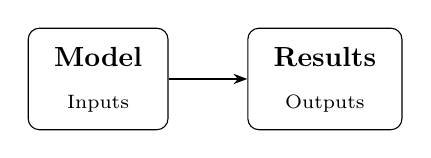
\begin{tikzpicture}
\node[box](a){\boxtext{Model}{Inputs}};
\node[box,right=of a](b){\boxtext{Results}{Outputs}};
\draw[arr](a)--(b);
\end{tikzpicture}}
\caption{Validation diagram.}\label{fig:validation}
\end{figure}
Figure~\ref{fig:validation} must resolve.
\begin{table}[H]\caption{Validation table.}\begin{tabularx}{\linewidth}{LL}
\toprule Input & Output \\\midrule Flow & Temperature \\\bottomrule
\end{tabularx}\end{table}
\begin{enumerate}\item First step.\item Second step.\end{enumerate}
\begin{thebibliography}{1}\small\bibitem{sample}LATFS. \url{https://latfs.duckdns.org}\end{thebibliography}
\end{document}
